\chapter{Fundamentação Teórica}
\label{fundamentacao}
Nesta seção são abordados os conceitos fundamentais utilizados neste trabalho e necessários para melhor entendimento do experimento.

\section{Classificação de Redes}
\label{classRedes}
Segundo Tanembaum, em \cite{tanembaum2011}, redes de telecomunicações são classificadas, comumente, de acordo com sua escala de abrangência. A seguir são apresentadas algumas das classificações de redes sem fio (figura \ref{fig:tecnologias_redes_semfiof}) mais relevantes para o escopo deste trabalho.

\begin{figure}[ht]
      \begin{center}
            \caption{Tecnologias de Redes Sem Fio}
            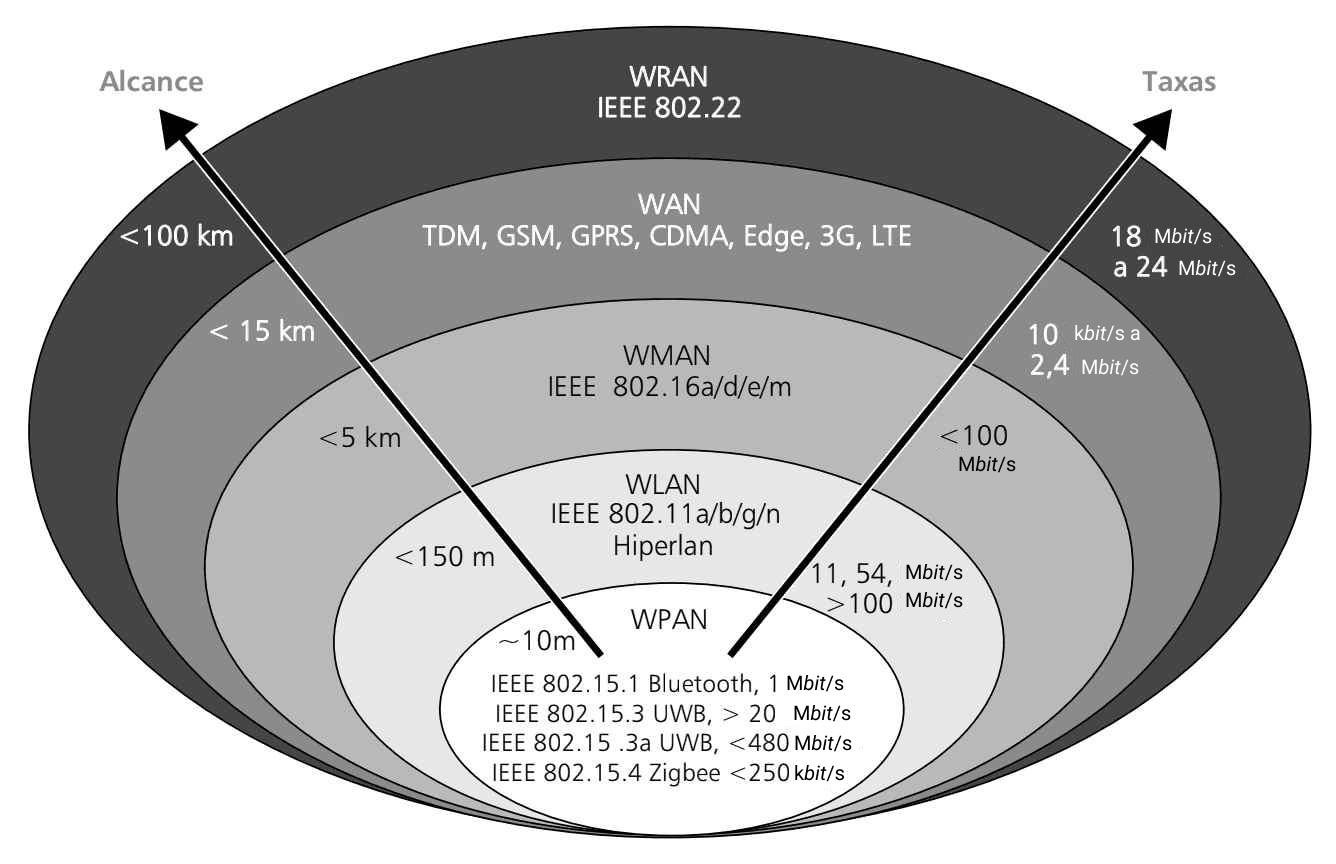
\includegraphics[width=10cm]{./sections/textual/chapters/images/tecnologias_redes_semfio.png}\\
            Imagem retirada do livro Sistemas de Comunicação Sem Fio \cite{rochol2018sistemas}.
            \label{fig:tecnologias_redes_semfiof}
      \end{center}
\end{figure}

\subsection{Classificação de Redes Sem Fio: Escala de Abrangência}
\subsubsection*{Redes sem fio pessoais - WPAN}
Inicialmente estas redes foram definidas para apresentar alcance limitado com a principal função de facilitar a conectividade de dispositivos periféricos ao computador ou telefone celular por uma conexão sem fio. O padrão IEEE 802.15 especifica a arquitetura destas redes sem fio, também denominadas \emph{piconets}. A principal  tecnologia comercial de redes WPAN é o Bluetooth (padrão IEEE 802.15.1).

O conceito de redes WPAN foi expandido para designar qualquer tipo de rede sem fio que atua em área restrita interconectando dispositivos, periféricos, atuadores ou um conjunto de sensores, geralmente com a capacidade de se auto-organizarem. E a partir dessa expansão é possível aplicações como redes de sensores sem fio, sistemas anticolisão e de condução automática em veículos, automação industrial, prédios inteligentes e monitoração de pacientes. Geralmente, estas redes utilizam a tecnologia ZigBee(IEEE 802.15.4) para a implementação da comunicação de rádio \cite{rochol2018sistemas}.

\subsubsection*{Redes Sem Fio Locais - WLAN}
São redes com a finalidade de conectar computadores de domésticos, de escritórios ou prédios em uma rede privada. Nesse tipo de rede, a tecnologia Wi-Fi(padrão IEEE 802.11) se tornou popular sendo adotado praticamente em todo computador e dispositivos moveis como \emph{smartphones} e \emph{tablets}.

Atualmente o padrão IEEE 802.11 utiliza de duas faixas de frequência não licenciada ISM, Industrial, Cientifica e Médica(Industrial, Scientific and Medic), as faixas em torno de 2,4GHz e 5GHz. Esta ultima faixa de frequência foi adicionada para garantir maiores taxas de transmissão. Como utiliza uma faixa de frequência não licenciada, é comum ocorrer interferência com outras redes Wi-Fi e com redes formadas por outras tecnologias que atuam na mesma faixa de frequências como Bluetooth e ZigBee \cite{rochol2018sistemas}.

\subsubsection*{Redes Celulares de Telefonia e Dados}
Estas redes abrangem diversos sistemas de telefonia conectados e ganharam bastante popularidade nas últimas décadas devido, principalmente, à redução de custos e aumento nas taxas de transmissão oferecidas pelas operadoras. Exemplos mais recentes de telefonia celular são GSM, EDGE e LTE que fornecem a segunda, terceira e quarta geração(2G, 3G e 4G) de telefonia celular, respectivamente.

Como abordado na seção \ref{padrõesSF}, há aplicações que utilizam infraestrutura GSM e LTE para aplicações de RSSF \cite{rochol2018sistemas}.


\subsubsection*{Redes de Longa Distância com Baixo Consumo Energético - LPWAN}
Em algumas aplicações IoT há requisitos muito específicos como atuação por uma grande extensão, dispositivos que possam passar longos períodos utilizando baterias e um bom custo beneficio. Tecnologias como ZigBee e Bluetooth não apresentam grande área de cobertura. Aplicações de telefonia celular apesar de grandes areas apresentam alto consumo energético.  Então, aplicações IoT impulsionaram a criação de novos padrões e tecnologia para um novo tipo de rede denominada de redes de longa distância com baixo consumo energético ou \emph{Low Power Wide Area Network}(LPWAN).

Dispositivos que implementam redes de baixo consumo energético ganharam popularidade na indústria e nas comunidades de pesquisa pois estabelecem comunicação sem fio de longas distâncias, de centenas de metros até alguns poucos quilômetros, com baterias que podem durar anos com uma única carga \cite{mekki2019comparative}.

A utilização desse tipo de rede se tornou fundamental para a implementação de RSSFs, oferecendo confiabilidade e baixo custo de implantação e manutenção. Na seção \ref{padrõesSF} são apresentados alguns dos principais padrões e tecnologias utilizadas nessas redes.

\section{Modelo de Camadas OSI}
\label{osi}
O modelo de referência para Interconexão de Sistemas Abertos, \emph{Open Systems Interconnection}, ou apenas modelo OSI, foi um passo para a padronização de redes de computadores. No modelo há sete camadas com funções bem definidas. A comunicação entre camadas é abstraída e se dá através de interfaces, ou seja, uma camada não tem acesso direto às camadas subjacentes, informação chega até ela no padrão pré-definido.

Para este trabalho será mais relevante a apresentação apenas das camadas 1 e 2 (figura \ref{fig:modelo_osi_1e2})  física e de enlace, respectivamente, e suas subcamadas do modelo OSI de forma generalizada de acordo o apresentado por Tanembaum em \cite{tanembaum2011} e por Rochol em \cite{rochol2018sistemas}.

\begin{figure}[ht]
      \begin{center}
            \caption{Camada Física e Camada de Enlace do Modelo OSI}
            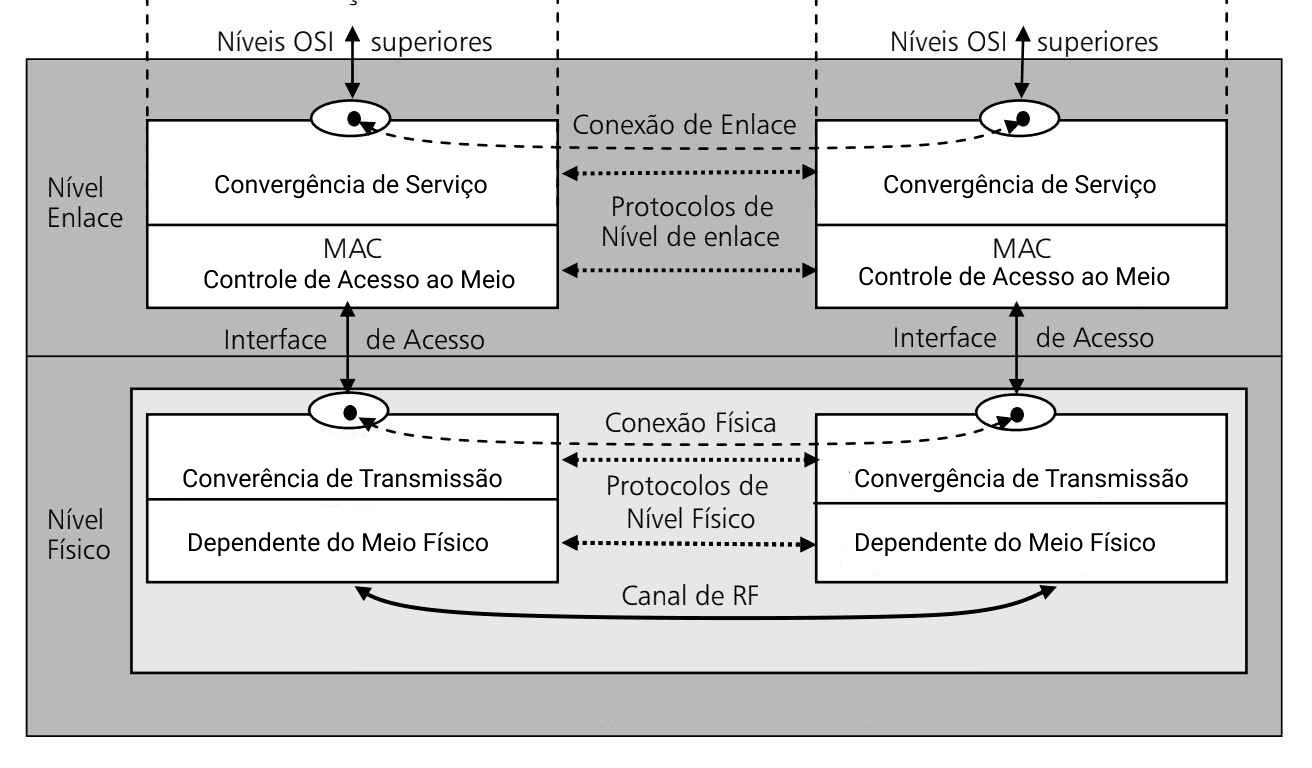
\includegraphics[width=10cm]{./sections/textual/chapters/images/modelo_osi_1e2.png}\\
            Imagem retirada do livro Sistemas de Comunicação Sem Fio \cite{rochol2018sistemas}.
            \label{fig:modelo_osi_1e2}
      \end{center}
\end{figure}


\subsection{Camada Física}
A camada física, de acordo \cite{tanembaum2011}, é uma abstração do meio físico de comunicação por onde trafegam os sinais do transmissor para o receptor definindo que sinais utilizar para os \emph{bits} 0 e 1; a duração de um bit; se a transmissão pode ser realizada nos dois sentidos ao mesmo tempo ou um de cada vez. De acordo Rochol em \cite{rochol2018sistemas} são consideradas duas sub-camadas: de convergência de transmissão do nível físico e a sub-camada dependente do meio.

Na sub-camada de convergência de transmissão é feita a codificação de canal, para obter confiabilidade na transmissão dos dados mesmo considerando as características problemáticas do canal de rádio frequência. Algumas funções implementadas nessa camada são descritas a seguir:
\begin{itemize}
      \item Embaralhamento do fluxo de \emph{bits}:

            Garante que os \emph{bits} 1 e 0 tenham a mesma probabilidade antes de serem enviados para transmissão. Ao realizar essa função, a utilização do canal é otimizada.
      \item Controle de erros:

            Utilização de técnicas para detectar e corrigir erros da transmissão. Por exemplo, adicionando alguns \emph{bits} à mensagem original e utiliza-los para detectar se algum bit da mensagem original foi modificado, podendo ser necessário uma retransmissão, ou talvez corrigir a mensagem recebida.
      \item Entrelaçamento de \emph{bits}:

            Uma técnica que utiliza algoritimos de distribuição temporal dos \emph{bits} da mensagem para espalhar a concentração de erros ao longo da sequência de \emph{bits}. Tornando mais eficiente a utilização das técnicas de controle de erros. Esses algorítimos são pré-definidos no transmissor e no receptor.
\end{itemize}

A segunda sub-camada da camada física corresponde às funcionalidades do transceptor de dados que depende do meio em que são implementadas. Transceptores mais simples, como modems ou regeneradores de sinais, utilizam protocolos e modulações para a transmissão/recepção do sinal mais simples como a codificação por pulsos. E alguns transceptores mais complexos que permitem maiores taxas de transmissão, múltiplos usuários e maior robustez a efeitos negativos no sinal rádio, possuem sistemas, geralmente com vários subsistemas, mais complexos utilizando diversos esquemas de modulação ao mesmo tempo, por exemplo o esquema de modulação OFDM, \emph{Orthogonal Frequency Division Multiplexing}(Multiplexação Ortogonal por Divisão de Frequência).


Há várias técnicas de transmissão e recepção de dados, porém, é possível agrupá-las em três classes, que são apresentadas a seguir em ordem crescente de complexidade:
\begin{enumerate}
      \item Técnicas de codificação por pulsos(ou modulação de banda base);
      \item Processos de modulação de um ou mais parâmetros de portadora única;
      \item Processo de modulação e transmissão utilizando múltiplas portadoras. Essas portadoras podem ser caracterizadas no domínio da frequência, utilizando múltiplas portadoras do tipo OFDM, Multiplexação por Divisão em Frequências Ortogonais. Ou podem ser caracterizadas no domínio do tempo como como ocorre no CDMA, Acesso Múltiplo por Divisão em Código, em que diferentes códigos ortogonais são aplicados simultaneamente sobre uma portadora digital gerando vários espectros ao redor de uma única portadora analógica, técnica também conhecida como espalhamento espectral.
\end{enumerate}

\subsection{Camada de Enlace}
A principal função implementada nessa camada, segundo Rochol em \cite{rochol2018sistemas}, é aumentar a garantia de que os \emph{bits} trafeguem na camada física livre de erros de transmissão. Esta camada faz com que o transmissor separe os dados e transmita cada parte de forma sequencial. Caso algum destas partes, ou quadros, da mensagem apresente erro, então pode ser retransmitida. Na camada de enlace há duas sub-camadas: de convergência de serviço e de acesso ao meio.

A sub-camada de convergência de serviço estabelece os requisitos de Qualidade de Serviço, \emph{Quality of Service}(QoS), da aplicação, como taxa de transmissão, atraso máximo de pacotes e taxa minima de perda de pacotes.

A sub-camada de de controle de acesso ao meio, ou \emph{Medium Access Control}(MAC), define como é feito o acesso ao meio de comunicação e, dependendo do protocolo utilizado, quem tem prioridade de utilização do meio. Há, principalmente, duas famílias de protocolos MAC utilizados em comunicações sem fio, ALOHA e CSMA, Acesso Múltiplo com Detecção de Portadora(\emph{Carrier Sense Multiple Access}).

O protocolo ALOHA define que os dados dos usuários devem ser transmitidos, mesmo que cause colisões de pacotes, porém, ao transmitir, o usuário deve sensorear o canal durante a transmissão e retransmitir a mensagem, caso seja percebido, por parte do transmissor, se houve colisão ou se o receptor da mensagem não confirmou o seu recebimento. Uma variação desse protocolo, chamado de \emph{Slotted} ALOHA foi desenvolvido com a intenção de diminuir a probabilidade de colisão dividindo o tempo em intervalos discretos de tempo, \emph{time slots}, exigindo sincronia entre todos os integrantes da rede para transmitir apenas nos intervalos certos.

O protocolo CSMA evita colisão de pacotes no canal. Para tal o transmissor tem que sensorear o canal antes de realizar uma transmissão. Caso o canal esteja livre, a transmissão é realizada. Caso o canal esteja ocupado, o transmissor espera até que esteja livre para transmitir ou transmite após um intervalo aleatório.


\section{Problemas da Comunicação Sem Fio}
Redes sem fios apresentam algumas vantagens em relação às redes cabeadas, por exemplo, facilidade de implementação e manutenção, flexibilidade, custos reduzidos e rapidez de implementação. Porém, o meio por onde as ondas de rádio são propagadas apresenta diversos desafios. O canal de radiofrequência pode apresentar, além do sinal do transmissor, sinais de estações transmissoras próximas, resíduos de transmissões passadas ou resíduos de efeitos térmicos do próprio transmissor, além, é claro, da forma como as ondas eletromagnéticas se propagam no meio, que pode ser um problema para recepção do sinal.

A seguir são apresentados alguns dos principais problemas para a recepção de sinais de rádio:

\subsection*{Ruído}
Em \cite{rochol2018sistemas} são apresentados dois tipos de ruídos: ruído branco ou ruído térmico e ruído impulsivo. Ruído térmico é caracterizado como a agitação molecular nos condutores e dispositivos físicos que realizam o processamento do sinal até a antena. Este tipo de ruído é impossível de ser eliminado completamente e limita o canal de radiofrequência; Ruído impulsivo é gerado por descargas atmosféricas ou equipamentos elétricos, que não são dispositivos de comunicação via rádio, próximos ao transmissor ou receptor, é imprevisível e de difícil controle, por exemplo, maquinas industriais e fornos micro-ondas, este que gera ruídos na faixa de 2,4GHz. Este tipo de ruído gera sequências de erros na transmissão, mecanismos de controle de erro dificilmente irão corrigir devido a alta concentração de erros.

\subsection*{Interferência}
Interferência, segundo Rappaport em \cite{rappaport2009}, é o maior fator limitante no desempenho de sistemas de rádio. Há dois tipos principais de inferência geradas pelo próprio sistema de rádio que são a interferência co-canal e a interferência de canal adjacente. Há também a interferência externa, gerada por dispositivos comunicação que utilizam das mesmas faixas de frequência utilizados pelo sistema, por exemplo, na faixa ISM em torno das frequências 2,4GHz há uma sobrecarga pois as tecnologias como Bluetooth e Wi-Fi operam nesta faixa. Interferência co-canal, segundo \cite{rochol2018sistemas}, é gerada, principalmente, em sistemas com múltiplos usuários que utilizam o mesmo canal. No caso de sistemas telefônicos, isto pode resultar em ligações cruzadas, em que usuários podem receber as informações de outras chamadas \cite{rappaport2009}. A interferência de canal adjacente ocorre quando uma transmissão é realizada muito proxima de um receptor que está recebendo transmissões de um outro transmissor. A recepção é prejudicada podendo se tornar inviável durante a transmissão do transmissor proximo ao receptor \cite{rappaport2009}.


\subsection*{Propagação por Múltiplos Caminhos}
Segundo Rochol em \cite{rochol2018sistemas} ao ser irradiado pela antena, a onda eletromagnética do sinal de rádio sofre inúmeras reflexões em obstáculos ao longo da sua trajetória até chegar ao receptor. Esse fenômeno é denominado de propagação por múltiplos caminhos. Este fenômeno explica três tipos de distorções observadas na transmissão por ondas de rádio: desvanecimento, espalhamento de atraso e espalhamento de Doppler.

O desvanecimento é causado quando várias cópias de um sinal, que percorreram vários caminhos, chegam à antena receptora com diferenças de fase, que fazem se somarem de forma destrutiva, causando uma recepção de má qualidade do sinal original, este efeito pode também gerar áreas de sombra do sinal. Os diversos sinais refletidos podem também se somar de forma construtiva melhorando a recepção do sinal em alguns pontos do espaço.

O espalhamento de atraso ocorre quando o sinal irradiado pela antena percorre caminhos diferentes e chegam ao receptor em intervalos diferentes. Fazendo com que a recepção do sinal seja duplicada ou ocorra uma interferência destrutiva como no caso do desvanecimento.

No espalhamento de Doppler é observado uma diferença na frequência da portadora e é causado principalmente pela mobilidade do receptor em relação ao transmissor. Quando o receptor está se movendo, aumenta a quantidade de percursos que o sinal pode percorrer e fatores como frequência da portadora, velocidade, prédios e carros podem influenciar na ocorrência do efeito Doppler.


\subsection*{Sombreamento}
O efeito de sombreamento é definido como áreas onde sinal recebido apresenta baixa potência devido a obstruções entre o transmissor e o receptor onde a recepção dos sinais acontece principalmente, por reflexões do sinal, sendo que os múltiplos caminhos que o sinal pode percorrer para chegar no local do receptor, podem ter uma efeito negativo na recepção do sinal.


\section{Padrões e tecnologias de comunicação para redes LPWAN}
\label{padrõesSF}
Segundo Tanembaum em \cite{tanembaum2011}, sem coordenação e cooperação entre fabricantes de dispositivos, não seria possível a interoperabilidade de sistemas. Sistemas IoT, como demonstrado em \cite{sotres2017practical}, podem ser constituídas de sistemas com vários dispositivos diferentes. Portanto, a padronização das telecomunicações são imprescindíveis, permitindo que dispositivos de diferentes fabricantes consigam se comunicar, não importando quem produziu a placa de rede, os cabos, roteadores ou comutadores.

\subsection{LoRa}
LoRaWAN, abreviação para \emph{Long Range Wide Area Networks}, é uma tecnologia que utiliza a implementação de camada física LoRa e protocolos de acesso ao meio. Utiliza uma técnica de modulação proprietária da SemTech baseada na técnica de modulação CSS, \emph{Chirp Spread Spectrum}. Essa técnica espalha um sinal de faixa estreita em um canal de banda larga, tornando o sinal mais resistente a interferências, mais difícil de se detectar por outros dispositivos que estejam sensoreando o canal de comunicação e mais resistente a obstruções no canal de comunicação. Utiliza as faixas ISM de 868 MHz, 915MHz e 433MHz na Europa, América do Norte e Asia, respectivamente. A taxa de transmissão pode variar de 300 \emph{bit}/s a até 50 k\emph{bit}/s, dependendo do fator de espalhamento utilizado na comunicação. A carga útil máxima de uma mensagem é 243 \emph{bytes} \cite{mekki2019comparative}.

A tecnologia LoRa é desenvolvida pela empresa estadunidense SemTech e o padrão LoRaWAN é mantido pelo consórcio de empresas chamado \emph{LoRa Alliance}.

\subsection{NB-IoT}
NarrowBand IoT é uma tecnologia especificada na versão 13 do 3GPP. Esta tecnologia opera na faixa de frequência celular(LTE e GSM), modulando os sinais utilizando a técnica QPSK, \emph{Quadrature Phase Shift Keying}(Modulação por Deslocamento de Fase em Quadratura). Utiliza faixas de frequência não ocupadas no LTE. Seu protocolo é uma versão simplificada do protocolo LTE, com menos funcionalidades que o LTE, para melhor se adequar sua utilização para IoT. Por exemplo, funções como monitoramento da qualidade do sinal ou conectividade dupla não são utilizadas, visando diminuir o uso de energia e aumentar a vida útil da bateria. Apresenta taxa de transmissão máxima de 200 k\emph{bits}/s e sua carga útil máxima é de 1600 \emph{bytes}.

\subsection{SigFox}
SigFox é uma tecnologia que não possui padronização oficial e é mantida pela empresa homônima. Os nós finais conectados a esta rede enviam para as estações radio base mensagens utilizando a modulação BPSK, \emph{Binary Phase Shift Keying}(Modulação por Deslocamento de Fase Binaria) utilizando bandas de frequência ultra-estreitas, até 100 Hz, na faixa de frequência ISM. Como utiliza uma faixa de frequência ultra estreita é eficiente energeticamente e resistente à interferência. Porém, não apresenta oferecer taxas de transmissão acima de 100 \emph{bit}/s.

A empresa SigFox oferece uma solução com conectividade ponta a ponta, o que significa que os dados entre o nó final são transmitidos para as estações rádio-base e vão diretamente para os servidores da empresa. Sendo possível apenas o envio de 140 mensagens por dia e cada mensagem enviada pode ter um payload máximo de 12 \emph{bytes}.

\subsection{IEEE 802.15.4}
No padrão IEEE 802.15.4 são definidas camadas físicas e de acesso ao meio utilizando as faixas ISM abaixo de 1GHz e 2,4 GHz, com as modulações BPSK e O-QPSK, Offset Quadrature Phase Shift Keying(Modulação por Deslocamento de Fase em Quadratura Deslocada), respectivamente. Com taxa de transmissão máxima de 250 k\emph{bit}/s utilizando a faixa de frequência de 2,4 GHz com um tamanho máximo de payload de 127 \emph{bytes} \cite{munoz2018overview} \cite{gomes2017estimaccao}. Este padrão é utilizado como base do ZigBee.

\subsection*{Emenda IEEE 802.15.4g}
Em 2015 foi proposta uma revisão do padrão IEEE 802.15.4 com novos esquemas de modulação com parâmetros de operação predefinidos para permitir uma melhor troca de faixa de comunicação, ocupação da largura de banda, taxa de transmissão de dados e confiabilidade da comunicação para melhor se adequar aos requisitos de diferentes aplicações. Assim, foi definido o padrão IEEE 802.15.4g que inclui as modulações SUN, \emph{Smart Utility Network}(Redes de Utilidades Inteligentes) \cite{tuset2020reliability}.

A seguir é apresentada uma visão geral das modulações:

\subsubsection*{SUN-FSK}
A técnica de modulação digital FSK, \emph{Frequency Shift Keying}(Chaveamento de Mudança de Frequência), altera a frequência, mantendo a amplitude da portadora constante, e os \emph{bits} de informação são transmitidos por meio do chaveamento de diferentes frequências \cite{lathi2012}.

Foi incluída no padrão por sua eficiência e compatibilidade com sistemas legados. Apresenta 3 modos de operação para cada uma das faixas de frequência definidas no padrão e possui parâmetros de canal e de modulação, em que é possível definir o tipo de modulação, a largura de banda do canal e o índice de modulação. Estes parâmetros definem a taxa de transmissão de 50 k\emph{bit}/s a até 200 k\emph{bit}/s.

\subsubsection*{SUN-OQPSK}
Originalmente, no padrão IEEE 802.15.4 foi adicionada a técnica de modulação DSSS-OQPSK, \emph{Direct Sequence Spread Spectrum Offset Quadrature Phase Shift Keying}(Modulação por Deslocamento de Fase em Quadratura Deslocada com Espalhamento Espectral de Sequência Direta), que se trata de uma técnica de modulação que utiliza chaveamento de fase, em um ângulo de 90$^{\circ}$, do sinal da portadora para transmitir dois \emph{bits} por vez e em seguida utilizando a técnica de espalhamento espectral de sequência direta espalha o sinal em uma ampla faixa de frequência utilizando uma sequência aleatória de alta taxa de \emph{bits}. Essas técnicas visam aumentar a taxa de transmissão e aumentar a robustez da transmissão, principalmente, tornando o sinal resiliente a interferência de faixa estreita, ruídos e diminuindo os efeitos de desvanecimento por múltiplos caminhos \cite{goldsmith2005wireless}.

Essa modulação está presente no texto original do padrão e foi estendida nesta emenda para adicionar bandas de frequência e suportar diferentes fatores de espalhamentos para conseguir atingir taxas de transmissão entre 6,25 k\emph{bit}/s a até 500 k\emph{bit}/s.

\subsubsection*{SUN-OFDM}
O esquema de modulação de OFDM, \emph{Orthogonal Frequency Division Multiplexing}(Multiplexação Ortogonal por Divisão de Frequência), divide os dados a serem transmitidos em sub-canais ortogonais centrados em  sub-portadoras com frequências diferentes. Essas sub-portadoras são comprimidas em uma faixa de frequência de acordo com a largura de banda disponível. Como é possível enviar dados por cada uma das sub-portadoras, é possível também ter uma elevada taxa de transmissão. As frequências de cada sub-portadora se sobrepõem, cada delas é ortogonal às suas subjacentes, garantindo que não haja interferência entre elas \cite{rappaport2009}\cite{goldsmith2005wireless}.

Esta modulação consegue prover altas taxas de transmissão e maiores faixas de comunicação, enquanto consegue lidar com interferência e propagação por múltiplos caminhos. Utiliza diferentes esquemas de modulação e codificação para alternar entre modulações, como BPSK, QPSK e 16-QAM, e esquemas de repetição de frequência para prover uma faixa de taxa de transmissão entre 50 k\emph{bits}/s a até 800 k\emph{bits}/s em um canal com a largura de banda que varia entre 200kHz e 1,2MHz.

\subsubsection*{Diversidade de Modulação}
Segundo Rappaport em \cite{rappaport2009}, diversidade é uma técnica utilizada para compensar os danos da atenuação do canal melhorando a qualidade do enlace de comunicações sem fio sem alterar a interface aérea, sem aumentar a potência ou a largura de banda transmitida.

A ideia de diversidade é que diferentes sinais são enviados por diferentes caminhos e, portanto, dificilmente, sofreram das mesmas complicações, aumentando a probabilidade de receber um sinal com menor quantidade de erros \cite{goldsmith2005wireless}. Normalmente, são utilizadas técnicas de diversidade aumentando o número de antenas receptoras ou utilizando múltiplos canais de comunicação.

Como demonstrado pelos autores em \cite{gomes2020improving} é possível utilizar as diferentes modulações do padrão IEEE 802.15.4g SUN para criar um esquema de diversidade de modulação, ou seja, utilizar as diferentes modulações do padrão de acordo com as variações do ambiente ou enviar repetições da mensagem com mais de uma modulação, podendo melhorar a qualidade do enlace.

\section{Parâmetros para Avaliação da Confiabilidade do Enlace Sem Fio}
\label{paramSF}
Algumas métricas são utilizadas para medir a qualidade de um enlace sem fio, algumas estão mais relacionadas à camada física, como RSSI, \emph{Received Signal Strength Indicator}(Indicador da Força do Sinal Recebido) e CCA, \emph{Clear Channel Assessment}(Verificação do Canal Limpo), ou mais relacionadas a camada de aplicação como o PDR, \emph{Packet Delivery Ratio}, Taxa de Entrega de Pacotes. Estas métricas são detalhadas a seguir.
\subsection*{RSSI}
RSSI é uma medida da energia de um sinal de rádio recebido. O RSSI é um valor relativo e pode variar de acordo com a fabricante do transceptor de rádio \cite{UNDERSTANDING_RSSI}. O valor de RSSI é apresentado -100dB até 0dB, os maiores valores, próximos a 0dB, significam uma boa qualidade do sinal recebido e valores menores, próximos a 100dB, significa sinais de baixa qualidade.

\subsection*{PDR}
PDR é um indicador de camada de aplicação que relaciona a quantidade de pacotes recebidos pelo receptor com a quantidade de pacotes enviados pelo transmissor. Dependendo da aplicação, há uma taxa mínima de entrega de pacotes, por exemplo,  aplicações industriais de alta capacidade necessitam de um PDR superior a 99,9\%.

\subsection*{CCA}
CCA é uma forma de verificar o canal antes da transmissão, a fim de detectar se ele está em uso. Obtido a partir da verificação da energia no canal, é medido em dBm. Caso o valor medido esteja acima de um limiar pré-determinado o transmissor não pode transmitir e espera um tempo aleatório em milissegundos para verificar novamente o canal. Este parâmetro faz parte do protocolo CSMA, citado na Seção \ref{osi}.

\section{Trabalhos relacionados}
 {Em \cite{tuset2020dataset} os autores do artigo realizaram um experimento para analisar o comportamento das modulações SUN do padrão IEEE 802.15.4g em um cenário industrial. Em  \cite{munoz2018overview} os autores realizaram um estudo aprofundado sobre a modulação SUN-OFDM no ambiente predial, demonstrando, entre outras coisas, que a modulação SUN-OFDM nas faixas de frequência sub-GHz se é mais vantajosa de utilizar que a modulação OQPSK do padrão IEEE 802.15.4.}
